\section{UML Diagramme}
\label{sec:UMLDiagramme}

Quelle: Oose.de - Notationsübersicht UML \cite{UMLNotationsuebersicht}

\subsection{Klassendiagramm}
\label{sec:Klassendiagramm}

\begin{center}
	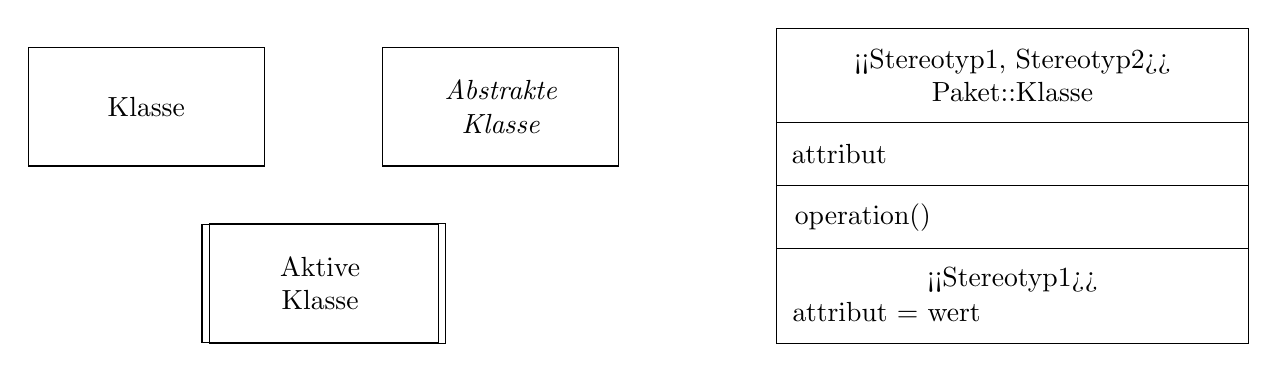
\begin{tikzpicture}[align=center]
		
		\draw (0,3) node[minimum height=1.5cm, minimum width=3cm, draw] {Klasse};
		\draw (4.5,3) node[minimum height=1.5cm, minimum width=3cm, draw, font=\itshape] {Abstrakte\\Klasse};
		
		\draw (0.7,0) node [minimum height=1.5cm, minimum width=3cm, anchor=south west, draw] {Aktive\\Klasse};
		\draw (0.8,0) rectangle (3.8,1.52);
		
		\draw (8,0) rectangle (14,4); 
		
		\node at (9.4,0.4){attribut = wert};
		\node at (11,0.8){<<Stereotyp1>>};
		\draw (8,1.2) -- (14,1.2);
		\node at (9.1,1.6) {operation()};
		\draw (8,2) -- (14,2);
		\node at (8.8,2.4) {attribut};
		\draw (8,2.8) -- (14,2.8);
		\node at (11,3.4) {<<Stereotyp1, Stereotyp2>>\\Paket::Klasse};
	\end{tikzpicture}
\end{center}

Sichtbarkeit:
\begin{multicols}{2}
	\begin{itemize}
		\item Öffentlich (+)
		\item Privat (-)
		\item Geschützt (\#)
		\item Paket (\textasciitilde)
		\item Abgeleitet (/)
		\item Statisch (unterstrichen)
	\end{itemize}
\end{multicols}

\vspace{2em}

\begin{tikzpicture}[align=center, node distance=4cm]
	\node[minimum height=1.5cm, minimum width=3cm, draw](vererbungklasse1){Klasse 1};
	\node[minimum height=1.5cm, minimum width=3cm, draw, right=of vererbungklasse1](vererbungklasse2){Klasse 2};
	\draw[-{Triangle[open]}, very thick] (vererbungklasse1) -- (vererbungklasse2) node[pos=.5,above]{Vererbung};
	
	\node[minimum height=1.5cm, minimum width=3cm, draw, below=1cm of vererbungklasse1](assoziationklasse1){Klasse 1};
	\node[minimum height=1.5cm, minimum width=3cm, draw, below=1cm of vererbungklasse2](assoziationklasse2){Klasse 2};
	\draw[very thick] (assoziationklasse1) -- (assoziationklasse2) node[pos=.5,above]{Assoziation};
	
	\node[minimum height=1.5cm, minimum width=3cm, draw, below=1cm of assoziationklasse1](gerichteteassoziationklasse1){Klasse 1};
	\node[minimum height=1.5cm, minimum width=3cm, draw, below=1cm of assoziationklasse2](gerichteteassoziationklasse2){Klasse 2};
	\draw[{Rays-to}, very thick] (gerichteteassoziationklasse1) -- (gerichteteassoziationklasse2) node[pos=.5,above]{gerichtete Assoziation};
	
	\node[minimum height=1.5cm, minimum width=3cm, draw, below=1cm of gerichteteassoziationklasse1](realisierungklasse1){Klasse 1};
	\node[minimum height=1.5cm, minimum width=3cm, draw, below=1cm of gerichteteassoziationklasse2](realisierungklasse2){Klasse 2};
	\draw[-{Triangle[open]}, very thick, dashed] (realisierungklasse1) -- (realisierungklasse2) node[pos=.5,above]{Realisierung};
\end{tikzpicture}


%\begin{minipage}[c]{0.65\textwidth}
%	\begin{itemize}
%		\item \textbf{Vererbung}: Prozess, bei dem eine Unterklasse die Eigenschaften einer Oberklasse übernimmt, wird auch als Generalisierung bezeichnet. Dargestellt durch eine gerade Verbindungslinie mit geschlossener Pfeilspitze, die auf die Oberklasse zeigt.
%	\end{itemize}
%\end{minipage}
%\hfill
%\begin{minipage}[c]{0.25\textwidth}
%	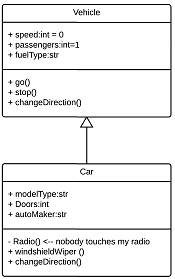
\includegraphics[scale=.7]{Bilder/Klassendiagramm/InteraktionVererbung.png}
%\end{minipage}

\subsection{Use-Case-Diagramm (Anwendungsfalldiagramm)}
\label{sec:UseCaseDiagramm}

\subsection{Aktivitätsdiagramm}
\label{sec:Aktivitaetsdiagramm}

\subsection{Sequenzdiagramm}
\label{sec:Sequenzdiagramm}

\subsection{Zustandsdiagramm}
\label{sec:Zustandsdiagramm}